\documentclass[mathNotesPreamble]{subfiles}
\begin{document}
%\relscale{1.4}
\section{3.11: Related Rates}
  \begin{thmBox*}
    Related rates are problems that use a mathematical relationship between two or more objects under specific constraints. From this, we can differentiate this relationship and examine how each variable changes with respect to time.
  \end{thmBox*}

\begin{ex*}
  An oil rig springs a leak in calm seas and the oil spreads in a circular patch around the rig. If the radius of the oil patch increases at a rate of $30m/hr$, how fast is the area of the patch increasing when the patch has a radius of $100 m$?
\end{ex*}
\vspace*{\stretch{0.4}}
\noindent
\textbf{Solution:}

\begin{center}
  \begin{minipage}{0.95\linewidth}
    We are given the radius $r=100\,m$ which is increasing at a rate of $\frac{dr}{dt}=30\,m/hr$. First, we note the formula for the area of a circle:
  \end{minipage}
  
  \vspace*{-5pt}
  \noindent
  \begin{minipage}[t]{0.65\linewidth}~
    \begin{align*}
      A&=\pi r^2\\
      \intertext{Now, we differentiate \textit{with respect to time} $t$:}
      \frac{dA}{dt}&=2\pi r\frac{dr}{dt}
    \end{align*}
  \end{minipage}%
  \begin{minipage}[t]{0.3\linewidth}~
    \begin{flushright}
      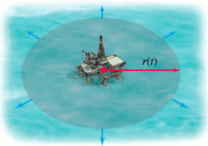
\includegraphics[width=\linewidth]{images/briggs_03_11/oilSpill.png}
    \end{flushright}
  \end{minipage}%
  
  \noindent
  \begin{minipage}{0.95\linewidth}
    Note that we want to solve for $\dfrac{dA}{dt}$ --- the rate of change of the area of the oil patch:
      $$\frac{dA}{dt}=2\pi\parens{100\,m}\parens{30\,m/hr}=6000\pi\, m^2/hr$$
  \end{minipage}
\end{center}
\vspace*{\stretch{1}}

\pagebreak
\begin{ex*}
  Two small planes approach an airport, one flying due west at $120\,mi/hr$ and the other flying due north at $150\, mi/hr$. Assuming they fly at the same constant elevation, how fast is the distance between the planes changing when the westbound plane is $180\,mi$ from the airport and the northbound plane is $225\,mi$ from the airport?
\end{ex*}
\vspace*{\stretch{0.4}}
\noindent
\textbf{Solution:}

\begin{center}
%  \begin{minipage}{0.95\linewidth}
%    Using the diagram below, we label the triangle formed between the planes and the airport such that the plane flying west is a distance of $x$ miles away from the airport, the plane flying north is $y$ miles away from the airport and the distance between the planes is $z$ miles.
%  \end{minipage}
  
  \noindent
  \begin{minipage}{0.6175\linewidth}~
  
    From the problem statement, we know that 
      \begin{align*}
        x&=180\,mi& y&=225\,mi\\
        \frac{dx}{dt}&=-120\,mi/hr& \frac{dy}{dt}&=-150\,mi/hr
      \end{align*}
      Now we use the Pythagorean theorem to relate the three sides:
      $$x^2+y^2=z^2$$
    Next, we differentiate and get the resulting relationship between the related rates:
      $$2x\,\frac{dx}{dt}+2y\,\frac{dy}{dt}=2z\,\frac{dz}{dt}$$
    Before we solve for $\frac{dz}{dt}$, we must find $z$:
  \end{minipage}%
  \begin{minipage}{0.33250\linewidth}~
    \begin{flushright}
      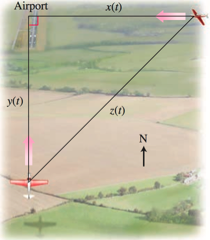
\includegraphics[width=0.95\linewidth]{images/briggs_03_11/airplane.png}
    \end{flushright}
  \end{minipage}
  
  \vspace*{5pt}
  \noindent
  \begin{minipage}{0.95\linewidth}
      $$z=\sqrt{180^2+225^2}=45\sqrt{4^2+5^2}=45\sqrt{41}\approx288\,mi$$
    This gives us
    \begin{align*}
      \frac{dz}{dt}
        =\frac{x\,\frac{dx}{dt}+y\,\frac{dy}{dt}}{z}
        &=\frac{\parens{180\,mi}\parens{-120\,mi/hr}+\parens{225\,mi}\parens{-150\,mi/hr}}{45\sqrt{41}\,mi}\\
        &=\frac{-1230}{\sqrt{41}}\,mi/hr\approx -192\,mi/hr
    \end{align*}
  \end{minipage}
\end{center}
\vspace*{\stretch{1}}
\pagebreak

\begin{thmBox*}[Steps for Related-Rate Problems]
  \begin{enumerate}
    \item Read the problem carefully, making a sketch to organize the given information. Identify the rates that are given and the rate that is to be determined.
    \item Write one or more equations that express the basic relationships among the variables.
    \item Introduce rates of change by differentiating the appropriate equation(s) with respect to time $t$.
    \item Substitute known values and solve for the desired quantity.
    \item Check that units are consistent and the answer is reasonable. (For example, does it have the correct sign?)
  \end{enumerate}
\end{thmBox*}

\textit{Note:} The \textit{Just-In-Time} book has some examples in chapter 14 that are helpful in setting up the relationships outlined in these types of word problems.
\pagebreak

\begin{ex*}
  A ladder 13 feet long rests against a vertical wall and is sliding down the wall at a constant rate of $3\,ft/s$. How fast is the foot of the ladder moving away from the wall when the foot of the ladder is $5\,ft$ from the base of the wall?
\end{ex*}
\pagebreak

\begin{ex*}
  The volume of a cube decreases at a rate of $0.5\,ft^3/min$. What is the rate of change of the side length when the side lengths are $12\,ft$?
\end{ex*}
\pagebreak

\begin{ex*}
  The length of a rectangle is increasing at a rate of $8\,cm/s$ and its width is increasing at a rate of $3\,cm/s$. When the length is $20\,cm$ and the width is $10\,cm$, how fast is the area of the rectangle increasing?
\end{ex*}
\pagebreak

\begin{ex*}
  A coffee mug has the shape of a right circular cylinder with inner diameter 4 inches and height 5 inches. If the mug is filled with hot chocolate at a constant rate of $2\,in^3/sec$, how fast is the level of the liquid rising?
\end{ex*}
\pagebreak

\begin{ex*}
  A rectangular swimming pool $10\,ft$ wide by $20\,ft$ long and of uniform depth is being filled with water.
\end{ex*}
\begin{enumerate}[label=\alph*), itemsep=\stretch{1}]
  %\item If $t$ is elapsed time, $h$ is the height of the water, and $V$ is the volume of the water, find equations relating $V$ to $h$ and $dV/dt$ to $dh/dt$.
  \item At what rate is the volume of the water increasing if the water level is rising at $\frac{1}{4}\,ft/min$?
  \item At what rate is the water level rising if the pool is filled at a rate of $10\,ft^3/min$?
\end{enumerate}
\vspace*{\stretch{1}}
\pagebreak

\begin{ex*}
  At all times, the length of a rectangle is twice the width $w$ of the rectangle as the area of the rectangle changes with respect to time $t$.
  \begin{enumerate}[label=\alph*), itemsep=\stretch{1}]
    \item Find the equation that relates $A$ to $w$.
    \item Find the equation that relates $dA/dt$ to $dw/dt$.
  \end{enumerate}
\end{ex*}
\vspace*{\stretch{1}}
\pagebreak

\begin{ex*}
  Assume $x,\, y$ and $z$ are functions of $t$ with $z=x+y^3$. Find $dz/dt$ when $dx/dt=-1,\ dy/dt=5$ and $y=2$.
  
\end{ex*}
\vspace*{\stretch{1}}

\begin{ex*}
  Assume $w=x^2y^4$, where $x$ and $y$ are functions of $t$. Find $dw/dt$ when $x=3,\, dx/dt=2,\,dy/dt=4$, and $y=1$.
\end{ex*}
\vspace*{\stretch{1}}
\pagebreak

\begin{ex*}
  The sides of a square decrease in length at a rate of $1\,m/s$.
\end{ex*}
\begin{enumerate}[label=\alph*), itemsep=\stretch{1}]
  \item At what rate is the area of the square changing when the sides are $5\,m$ long?
  \item At what rate are the lengths of the diagonals of the square changing?
\end{enumerate}
\vspace*{\stretch{1}}
\pagebreak

\begin{ex*}
  At noon bicyclist A is 25 miles south of an intersection and bicyclist B is 8 miles west of the same intersection. Bicyclist A is traveling north at 11 miles per hour and bicyclist B is traveling 6 miles per hour west of the intersection. How is the distance between riders changing at 2pm?
\end{ex*}
\pagebreak

\begin{ex*}
  A ladder 13 feet long rests against a vertical wall and is sliding down the wall at a constant rate of $3\,ft/s$. How fast is the angle between the top of the ladder and the wall changing when the angle is $\frac{\pi}{4}$ radians?
\end{ex*}
\pagebreak

\noindent
\begin{minipage}[t]{0.7\linewidth}\mbox{}
  \begin{ex*}[Piston compression]
    A piston is seated at the top of a cylindrical chamber with radius $5\,cm$ when it starts moving into the chamber at a constant speed of $3\,cm/s$. What is the rate of change of the volume of the cylinder when the piston is $2\,cm$ from the base of the chamber?
  \end{ex*}
\end{minipage}%
\begin{minipage}[t]{0.3\linewidth}\mbox{}
  \begin{flushright}
    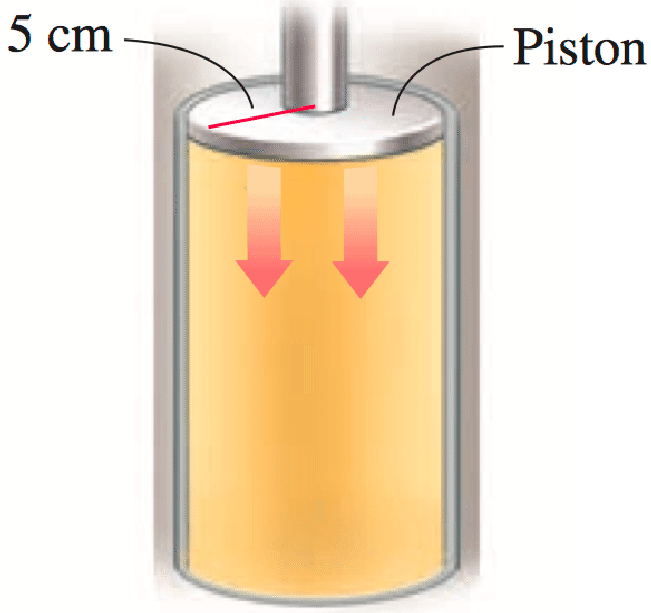
\includegraphics[width=0.9\linewidth]{images/briggs_03_11/piston.png}
  \end{flushright}
\end{minipage}
\pagebreak

\begin{ex*}
  Suppose we have a snowball that is a perfect sphere. If the snowball is melting at a rate of $5\,in^3/min$, how fast is the radius changing when the radius is 10 inches? How fast is the surface area changing?
\end{ex*}
\pagebreak

\noindent
\begin{minipage}[t]{0.7\linewidth}\mbox{}
  \begin{ex*}
    A dinghy is pulled toward a dock by a rope from the bow through a ring on the dock $6\,ft$ above the bow.  The rope is hauled in at a rate of $2\,ft/sec$. At what rate is the angle $\theta$ changing when 10 ft of rope is out?
  \end{ex*}
\end{minipage}%
\begin{minipage}[t]{0.3\linewidth}\mbox{}
  \begin{flushright}
    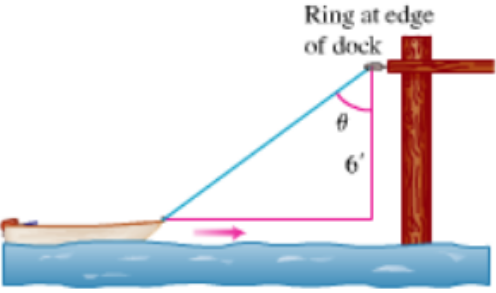
\includegraphics[width=0.9\linewidth]{images/briggs_03_11/dinghy.png}
  \end{flushright}
\end{minipage}
\pagebreak

\begin{ex*}
  At noon, ship A is $150\,km$ west of ship B. Ship A is sailing east at $35\,km/h$ and ship B is sailing north at $25\,km/h$. How fast is the distance between the ships changing at 4pm?
\end{ex*}
\pagebreak

\begin{ex*}
  Once Kate's kite reaches a height of $50\,ft$ (above her hands), it rises no higher but drifts due east in a wind blowing $5\,ft/s$. How fast is the string running through Kate's hands at the moment that she has released $120\,ft$ of string?
\end{ex*}
\pagebreak

\noindent
\begin{minipage}[t]{0.7\linewidth}\mbox{}
  \begin{ex*}
  Two carts, A and B, are connected by a rope $39\,ft$ long that passes over a pulley $P$. The point $Q$ is on the floor $12\,ft$ directly beneath $P$ and between the carts.  Cart A is being pulled away from $Q$ at  a speed of $2\,ft/s$.  How fast is cart B moving toward $Q$ at the instant when cart A is $5\,ft$ from $Q$?
\end{ex*}
\end{minipage}%
\begin{minipage}[t]{0.3\linewidth}\mbox{}
  \begin{flushright}
    \vspace*{7.5pt}
    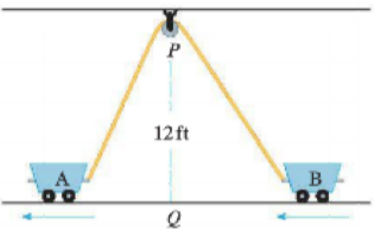
\includegraphics[width=0.9\linewidth]{images/briggs_03_11/cart.png}
  \end{flushright}
\end{minipage}%
\pagebreak

\begin{ex*}
   A camera is set up at the starting line of a drag race 50ft from a dragster at the starting line (camera 1 in the figure). Two seconds after the start of the race, the dragster has traveled 100ft and the camera is turning at 0.75rad/s while filming the dragster.
  \begin{enumerate}[label=\alph*)]
    \item What is the speed of the dragster at this point?
    \item A second camera (camera 2 in the figure) filming the dragster is located on the starting line $100\,ft$ away from the dragster at the start of the race. How fast is this camera turning $2\,s$ after the start of the race?
  \end{enumerate}
\end{ex*}
\vspace*{-20pt}
\begin{flushright}
  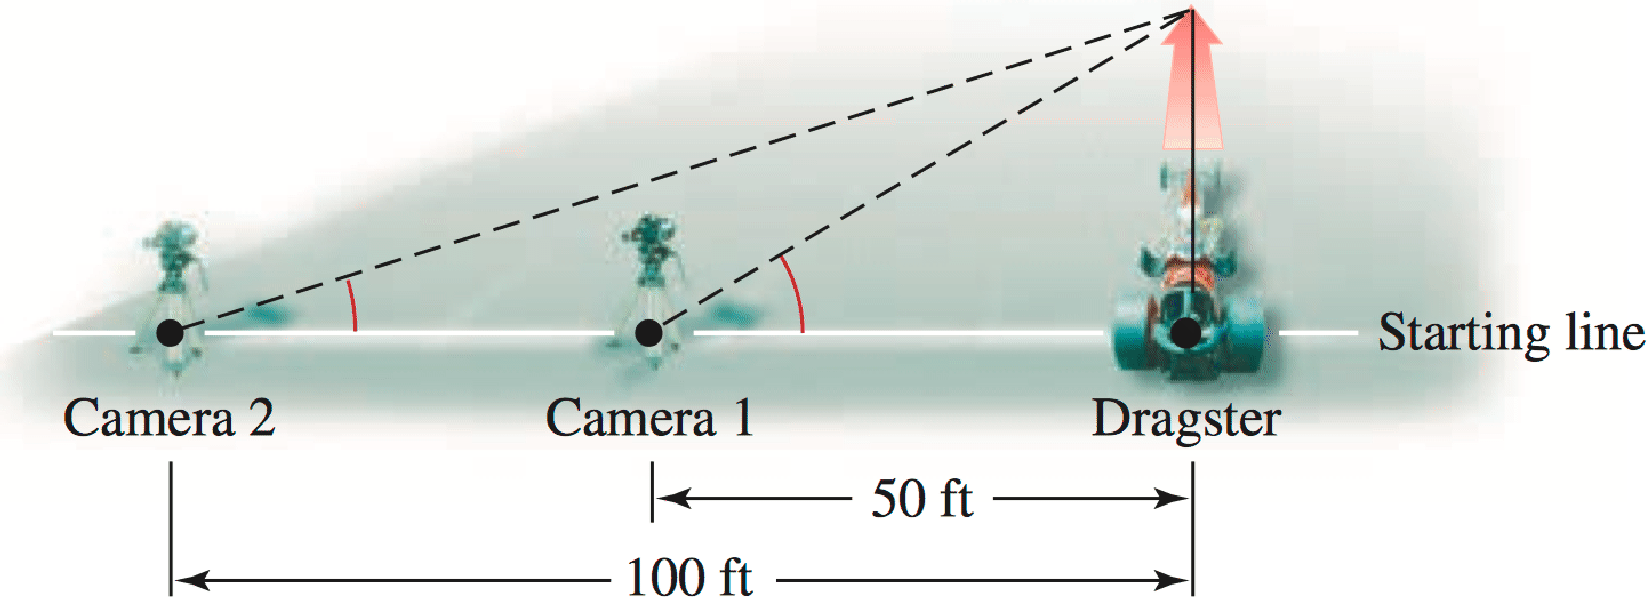
\includegraphics[width=0.5\linewidth]{images/briggs_03_11/dragrace.png}
\end{flushright}
\pagebreak

\begin{ex*}
  A television camera is positioned $4000\,ft$ from the base of a rocket launching pad.  The angle of elevation of the camera has to change at the correct rate in order to keep the rocket in sight. Also the mechanism for focusing the camera has to take into account the increasing distance from the camera to the rising rocket. Assume the rocket rises vertically and its speed is $600\,ft/s$ when it has risen $3000\,ft$. How fast is the distance from the television camera to the rocket changing at that moment? Also, if the television camera is always kept aimed at the rocket, how fast is the camera’s angle of elevation changing at that same moment?
\end{ex*}
\pagebreak
\end{document}